\documentclass[twocolumn]{aastex63}

% typography
\usepackage[T1]{fontenc}

\usepackage{amsmath}

\setlength{\parindent}{1.\baselineskip}
\newcommand{\acronym}[1]{{\small{#1}}}
\newcommand{\package}[1]{\textsl{#1}}
\newcommand{\gaia}{\textsl{Gaia}}
% \newcommand{\hst}{\textsl{HST}}
% \newcommand{\pans}{\textsl{Pan-STARRS}}

% \newcommand{\deg}{\ensuremath{\textrm{deg}}}
\newcommand{\kpc}{\ensuremath{\textrm{kpc}}}
\newcommand{\ul}{\ensuremath{\textrm{kpc}^2\,\textrm{Myr}^{-1}}}
\newcommand{\ue}{\ensuremath{\textrm{kpc}^2\,\textrm{Myr}^{-2}}}
\newcommand{\kms}{\ensuremath{\textrm{km}\,\textrm{s}^{-1}}}
\newcommand{\masyr}{\ensuremath{\textrm{mas}\,\textrm{yr}^{-1}}}
\newcommand{\feh}{\ensuremath{\textrm{[Fe/H]}}}
\newcommand{\afe}{\ensuremath{\textrm{[$\alpha$/Fe]}}}

\newcommand{\changes}[1]{{\textbf{#1}}}
\hyphenation{kruijs-sen}

% aastex parameters
% \received{not yet; THIS IS A DRAFT}
%\revised{not yet}
%\accepted{not yet}
% % Adds "Submitted to " the arguement.
% \submitjournal{ApJ}
\shorttitle{}
\shortauthors{bonaca et al.}

%@arxiver{} test

\begin{document}\sloppy\sloppypar\raggedbottom\frenchspacing % trust me

\title{Phase-space Clustering Identifies the Origin of Galactic Stellar Streams}

\correspondingauthor{Ana~Bonaca}
\email{ana.bonaca@cfa.harvard.edu}

\author[0000-0002-7846-9787]{Ana~Bonaca}
\affil{Center for Astrophysics | Harvard \& Smithsonian, 60 Garden Street, Cambridge, MA 02138, USA}

\author{coauthors}

% \author[0000-0002-8804-0212]{J.~M.~Diederik~Kruijssen}
% \affiliation{Astronomisches Rechen-Institut, Zentrum f\" ur Astronomie der Universit\" at Heidelberg, M\" onchhofstra\ss e 12-14, D-69120 Heidelberg, Germany}
% \affil{Center for Astrophysics | Harvard \& Smithsonian, 60 Garden Street, Cambridge, MA 02138, USA}


\begin{abstract}\noindent % trust me
Most stellar streams in the Milky Way lack a discernible progenitor.
With the vast improvement in the precision of proper motions provided by Gaia EDR3, we show that the orbits of 23 Galactic stellar streams are highly clustered in orbital phase space.
Based on their energies and angular momenta, all streams in our sample can plausibly be associated with a (disrupted) dwarf galaxy host that brought them into the Milky Way.
For XX streams we also identify likely globular cluster progenitors.
Surprisingly, these stream progenitors are displaced from their tidal debris by XX degrees.
Finally, we identify stellar streams that appear spatially distinct, but whose similar orbits indicate they likely originate from the same progenitor.
If confirmed as physical discontinuities, they will provide strong constraints on the mass-loss rate from the progenitor, and possibly regions of chaotic dispersal in the Galaxy.
The universal ex-situ origin of existing stellar streams makes them valuable tracers of galaxy mergers and dynamical friction.
Their phase-space clustering can be leveraged to construct a precise global map of dark matter in the Milky Way, while their structure may hold clues to the small-scale structure of dark matter in their original host galaxies.
% : Fimbulthul with Thamnos; GD-1, Gj\" oll, Leiptr, Phlegethon, Wambelong, and Ylgr with Sequoia / Arjuna / I'itoi; Ophiuchus with Gaia-Enceladus; Aliqa Uma, ATLAS, Elqui, Slidr, Sylgr, and Turranburra with Sagittarius; Fjorm, and Turbio with Helmi Streams; Indus, Jhelum, Phoenix, Ravi, and Sv\" ol with Wukong; and Triangulum and Willka Yaku with Cetus.
% (Omega Cen---Fimbulthul, NGC~3201---Gj\" oll, NGC~4590---Fjorm, NGC~5024---Sylgr and Ravi, NGC~5272---Sv\" ol, NGC~5824---Triangulum).
% - connected to gcs
% Frequent associations of streams to bound clusters may indicate a rapid dispersal following the full dissolution of the progenitor cluster, while 
% have orbits similar to those of surviving globular clusters, despite being spatially offset from them.
% their spatial offset is potentially a signature of episodic mass loss.
\end{abstract}

\keywords{%
stars:~kinematics~and~dynamics
  ---
Galaxy:~halo
  ---
Galaxy:~kinematics~and~dynamics
}

\section{Introduction}
\label{sec:intro}

%  - from CC: the Intro should be short!  2-3 P.

% - streams observed messed up

% - happened in the mw or inherited from the host?
% - can't tell since we don't know the origin

% - for stars and gc: ex-situ identified from their orbital properties

% - been hard for streams bc most stars faint, couldn't do good orbits
% - but then edr3 happened
% - present here elz for streams
Stellar streams in the halo --  ribbons of stars that crisscross the sky, often extending tens of degrees -- hold the promise of delivering fundamental insights about the Galaxy and the nature of dark matter. 
Due to their intrinsic dynamical coldness, even subtle gravitational perturbations leave prominent marks on their bodies (e.g., gaps due to encounters with dark matter subhalos, fans due to encounters with the bar) that may be mined for new physics \citep[e.g.,][]{bonaca2019a}.
However, almost every detailed study of a stellar stream has revealed an extremely messy picture, with complex morphologies, large velocity dispersions, and widths incommensurate with simple models \citep[e.g.,][]{li2020,bonaca2020b,malhan2019b}. 

The key missing piece of context in our modeling of streams is knowledge of their origins. 
We are still unable to answer the most basic of questions: were most streams born in-situ, or did they enter the Milky Way during mergers with dwarf galaxies?
Understanding the origin of streams is critical to fulfilling their promise as probes of fundamental physics. 
For instance, the velocity structure of a stream born in the MW will be markedly different from that of a stream accreted after several orbits around a dwarf galaxy. 
Details of the dwarf galaxy -- whether it was massive or puny, cored or cusped -- also leave imprints on stream velocities \citep[][]{malhan2020}. 
Other aspects of the dwarf host (e.g., its accretion redshift) can help bracket how long the stream must be orbiting the Milky Way for, and thus constrain crucial parameters like the expected number of subhalo encounters.

While a succession of \textit{Gaia}-aided studies has tagged virtually every halo GC and star to a distinct dwarf merger \citep[e.g.,][]{massari19,naidu2020}, the genealogy of streams is still elusive.
Stream orbits are too uncertain because the faintness of stream stars has made velocity information hard to come by.
The recent \textit{Gaia} EDR3 has pushed the proper motion frontier into the stellar stream regime, allowing us, for the first time, to reconstruct the history of the MW's stream population. 
With these PMs we can finally compute stream integrals of motion (e.g., energies, angular momenta) as has been done for GCs and stars to identify clustered objects that arrived in the MW together. Here we present integrals of motion (energy, angular momenta) for 23 MW streams (\S\ref{sec:streamorbits},\ref{sec:phasespace}), identify families of streams with common origins, associate them with disrupted dwarf galaxies or known GCs (\S\ref{sec:hosts}), and discuss the implications of our constructed stream ancestry tree (\S\ref{sec:discussion}).

% Hypotheses:
% \begin{itemize}
% \item{We can associate streams with the Milky Way progenitor galaxies.}
% \item{Streams are clumped at the center of the progenitor with which they were accreted. Streams were dissolved because they experienced stronger tidal field than clusters stripped out at higher energies (which is why they remain bound until today). This explains why streams are clumpy in the phase-space, while globular clusters are not.}
% \item{Strength of Milky Way's tidal field at this location equals the gravitational pull of the progenitor, which is why everything fell apart here. Therefore, we can read off the mass of the progenitor from this location, and compare that to the neural net estimates.}
% \item{The span in angular momentum (and energy?) of clusters and streams is set by dynamical friction the progenitor experienced, which provides another way to estimate the mass of the progenitor galaxy.}
% \item{The energy of the progenitor's center (stream clump) maps to the accretion redshift.}
% \item{A massive globular cluster close to a stream clump was likely this progenitor's nuclear star cluster.}
% \item{Given our better understanding of the trail a galaxy leaves in the phase space, we can also update globular cluster and stream associations previously reported. Based on that, it seems like we have another retrograde progenitor in addition to Sequoia!}
% \item{Based on their proximity in the phase space, at least some streams considered so far as individual objects, may in fact be different parts of the same structure.}
% \end{itemize}
% 
% Puzzles / spin-offs:
% \begin{itemize}
% \item{Why are both prograde and retrograde progenitors leaving trails like \textbackslash \textbackslash\ instead of \textbackslash\ /?}
% \item{It seems that there are some gaps in the phase space, both in the distribution of streams and clusters, and H3 stars. Are these just well-separated, distinct progenitors?}
% \item{Taking uncertainties into account, are the stream clumps actually distinct? (How strongly) Can we rule out a uniform distribution?}
% \item{Can we use metallicity of streams and field stars in this analysis? Do we expect it to follow the globular cluster trail?}
% \item{How are EMOSAICS clusters distributed in the phase space?}
% \end{itemize}

\section{Stream Orbits}
\label{sec:streamorbits}
In this work we use stream orbits derived by \citet{bk2021}, and in this section provide a brief overview of their fitting procedure.
Positions and velocities of stream stars trace the orbit of their progenitor \citep[e.g.,][]{kuepper2010}.
Thanks to data released by the \gaia\ mission, 3D positions and two proper motion components are known for a sample of 23 streams without a discernible progenitor \citep{ibata2019, shipp2019, riley2020}.
To improve upon published proper motions of Elqui, Phoenix, Turbio, Turranburra, and Willka Yaku, we selected blue horizontal branch stars along these streams in the Gaia EDR3 catalog and used them in orbit fitting.
Radial velocities have been measured for five of these streams for full 6D phase-space information \citep{caldwell2020, li2020, bonaca2020b}.

%minor: the omega-cen stream has RVs too from the Ibata Science paper page 24 here https://arxiv.org/pdf/1902.09544.pdf

Assuming a static, axisymmetric model of the Milky Way \citep[default \texttt{MilkyWayPotential}]{gala}, \citet{bk2021} used these stream data to constrain their orbits.
They sampled the stream orbital parameters using a Monte Carlo Markov Chain ensemble sampler and provide direct samples from the posterior to account for correlations between parameters.
In this work we characterize the orbit by its total energy, $E_{\rm tot}$, and the $z$ component of the angular momentum, $L_z$ (perpendicular to the Galactic disk)---both conserved quantities in the adopted gravitational potential.
We further employ the orthogonal component of the angular momentum $L_\perp = \sqrt{L_x^2 + L_y^2}$, which is not fully conserved in an axisymmetric potential, but is still a useful quantity for orbital characterization \citep{helmi1999}.
We use a right-handed coordinate system, such that $L_z<0$ denotes prograde orbits.

\begin{figure*}
\begin{center}
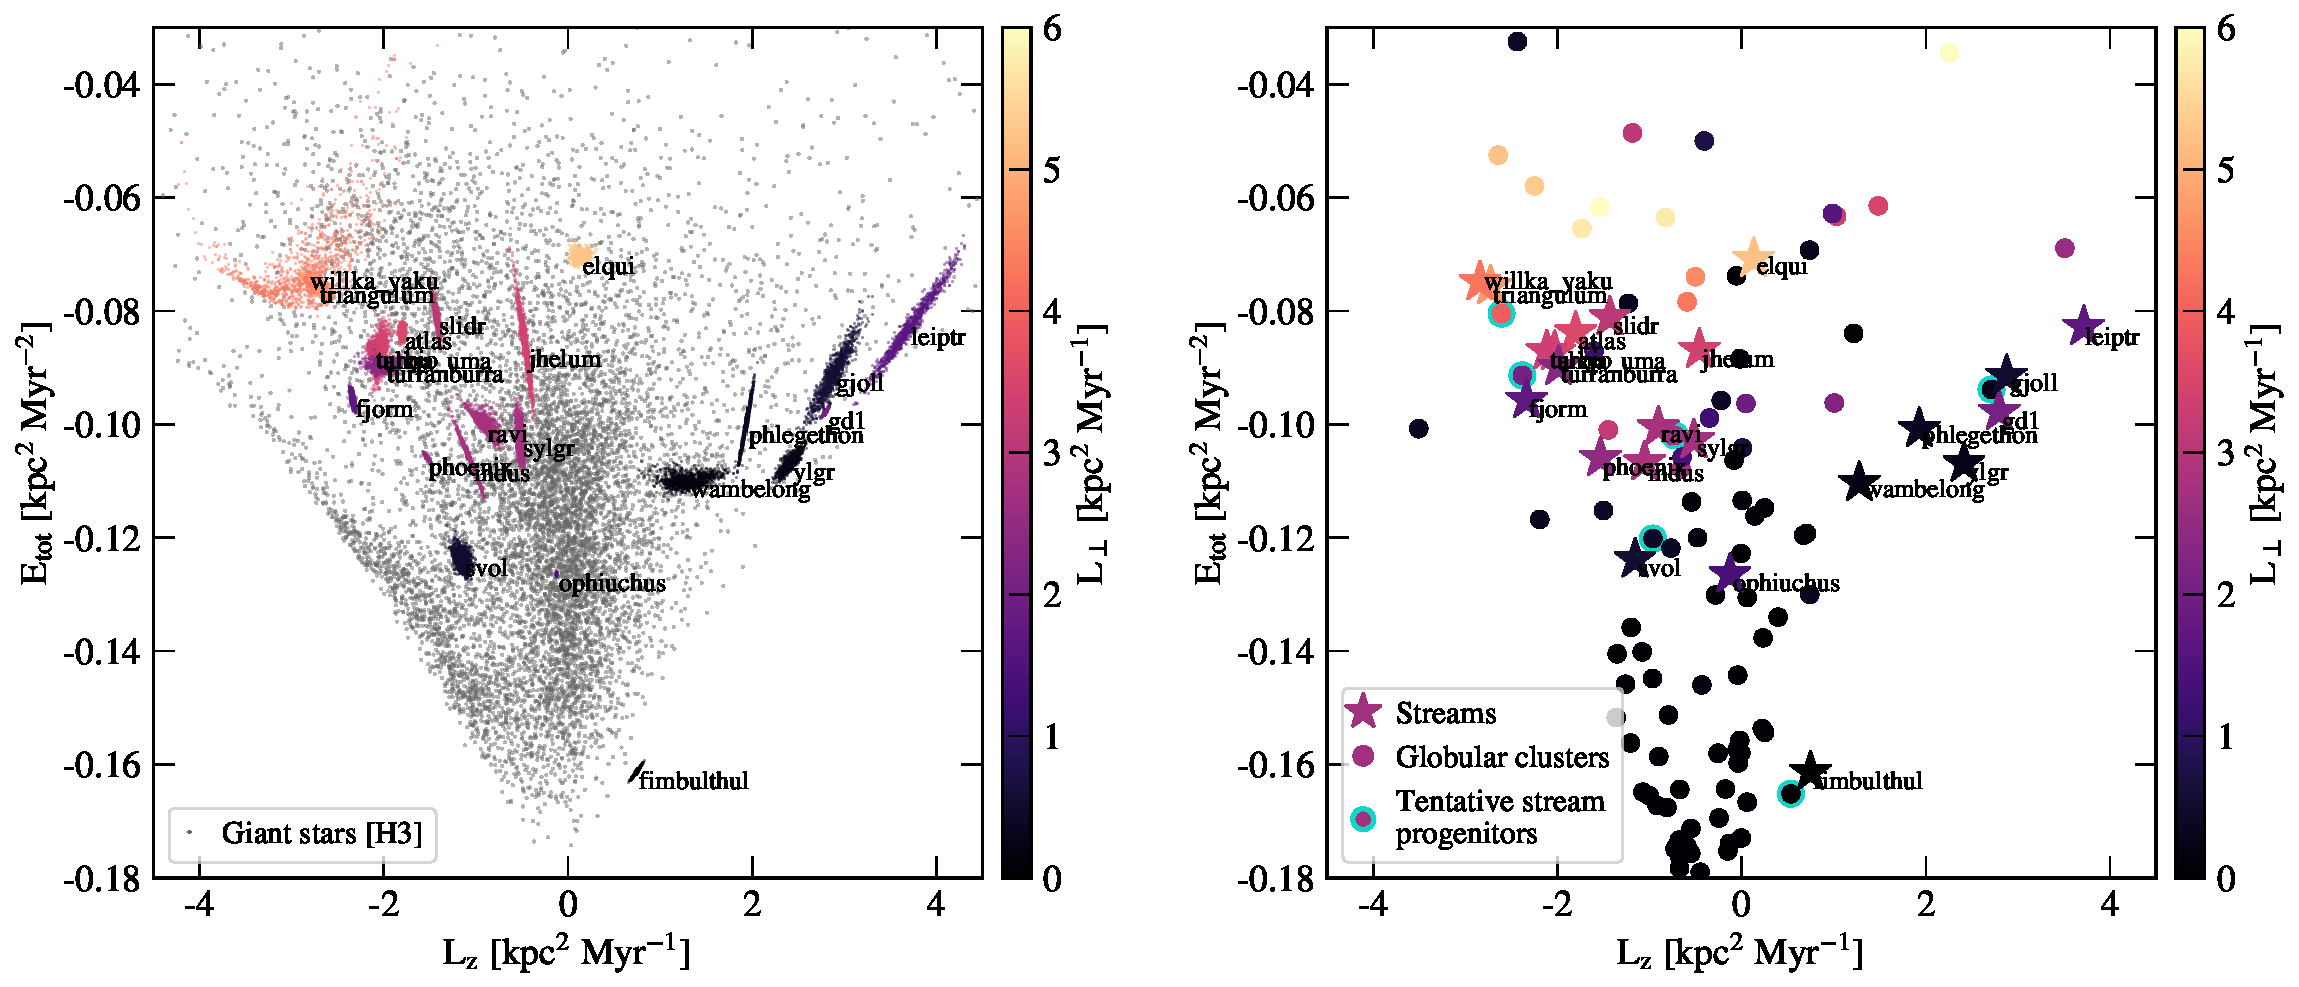
\includegraphics[width=\textwidth]{elz_streams.pdf}
\end{center}
\caption{The orbital phase space for cold stellar streams in the Milky Way (energy and angular momentum perpendicular to the disk, color-coded by the average orthogonal component of angular momentum), compared to field stars (left) and globular clusters (right).
Unlike stars and clusters, streams predominantly occupy tangential orbits and are more strongly clustered in phase space.
Globular clusters in close neighborhood of streams are plausible progenitors (cyan outlines).
}
\label{fig:elz}
\end{figure*}

\section{Streams in phase space}
\label{sec:phasespace}

\subsection{Overview}
\label{sec:elz}

We present the phase-space distribution of Galactic streams in Figure~\ref{fig:elz}.
In the left panel, each stream is represented in energy and $L_z$ angular momentum with 1000 samples from the posterior distributions, while the medians of these distributions are shown as stars in the right panel.
In both panels points are color-coded by the in-plane component of the angular momentum, $L_\perp$.
As a comparison, we include the phase-space distribution of giant stars from the H3 spectroscopic survey \citep[left panel, small black points;][]{conroy2019}, and Galactic globular clusters \citep[righ panel, small circles colored by $L_\perp$;][]{baumgardt2019}.

Interestingly, at the same amplitude of the angular momentum, $|L_z|$, prograde streams have higher energies than retrograde streams.
As spatial-overdensity searches are insensitive to the orbital direction, and proper-motion based searches are more sensitive to retrograde orbits, it is unlikely that the lack of retrograde streams at high energies is due to observational biases.
If confirmed as a reflection of the intrinsic orbital distribution by more complete stream samples, this asymmetry would suggest that objects on retrograde orbits are more resilient to tidal disruption, consistent with findings from numerical simulations \citep[e.g.,][]{find}.

The two most striking features of streams in the phase space are: (1) the significant degree of clustering, and (2) the lack of streams on radial orbits.
In contrast, the major feature in stars and globular clusters is the large population of objects on radial orbits with $L_z\approx0$, identified as debris from the Gaia Enceladus merger \citep[e.g.,][]{belokurov2018, helmi2018, naidu2020}.
Only two stellar streams are found on radial orbits, Ophiuchus and Elqui, and because of the large difference in their orbital energies they are likely unrelated.
Unlike stars and globular clusters, the majority of the streams are highly clustered in two groups, a retrograde group containing 7 streams, and a prograde group comprised of 14 streams.

Most of the retrograde streams are found on a narrow locus from $(E_{\rm tot}, L_z)\approx(-0.08\,\ue,\allowbreak 4\,\ul)$ to $(E_{\rm tot}, L_z)\approx(-0.11\,\ue,\allowbreak 1\,\ul)$, which includes Leiptr, Gj\" oll, GD-1, Phlegethon, Ylgr, and Wambelong.
Fimbulthul is on the extension of this diagonal to lower energies.
With the exception of GD-1 and Leiptr, all retrograde streams have uniformly low $L_\perp\lesssim1\,\ul$.
This clustering suggests that the entire retrograde group shares a common origin.  {\color{red} A "plane of streams"??}

The prograde group of streams appears to separate into three distinct regions: (1) Triangulum and Willka Yaku at $L_z\approx-3\,\ul$, (2) Slidr, ATLAS, Aliqa Uma, Turbio, Turraburra, and Fjorm at $L_z\approx-2\,\ul$, and (3) Jhelum, Sylgr, Ravi, Indus, Phoenix, and Sv\" oll at $L_z\approx-1\,\ul$.
The in-plane angular momentum decreases with decreasing $|L_z|$ and is approximately uniform within each small cluster.
The median energy of these sub-groups also decreases with decreasing $|L_z|$, however, so does the dispersion, such that the most radial clump spans a large range in energy levels.
Clustering of the prograde streams  provides tantalizing evidence of a common origin among stellar streams, which we explore further in \S\,\ref{sec:hosts}.

Several streams are also very closely associated with a globular cluster in phase space, suggesting a possible physical connection.
These clusters appear close to streams in energy and both components of the angular momentum, and are outlined in cyan in the right panel of Figure~\ref{fig:elz}.
The identified cluster--stream groups include: Omega Cen--Fimbulthul; NGC~3201--Gj\" oll; NGC~4590--Fjorm; NGC~5024--Sylgr and Ravi; NGC~5272--Sv\" ol; and NGC~5824--Triangulum.
We explore these connections further in \S\,\ref{sec:progenitors}.

\begin{figure*}
\begin{center}
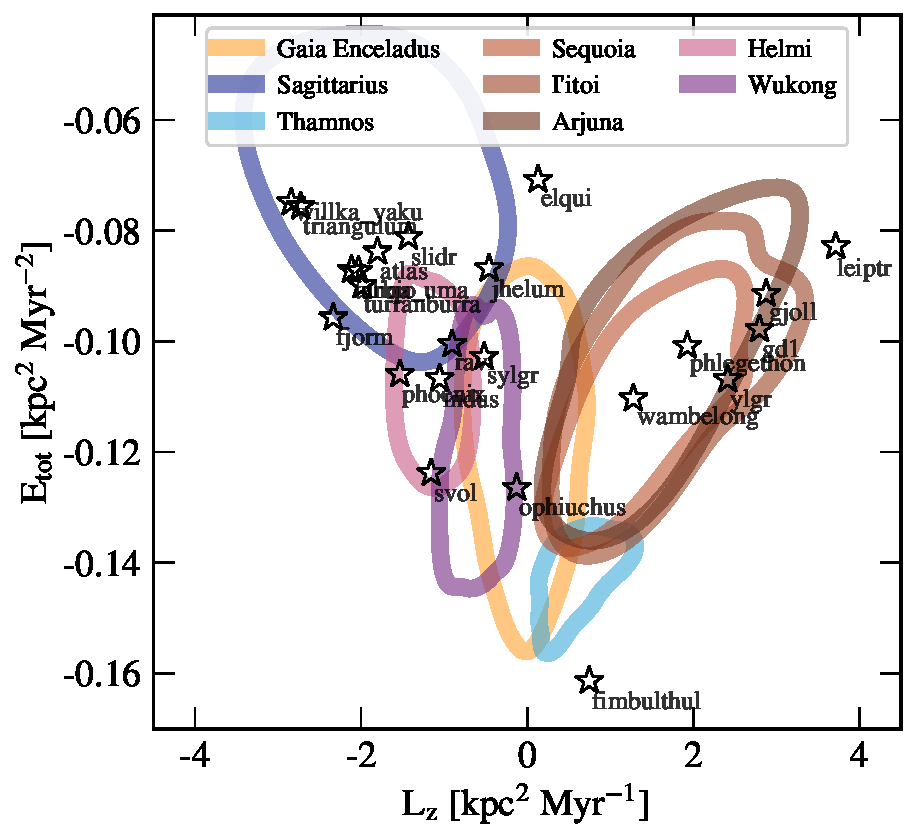
\includegraphics[width=\textwidth]{stream_hosts.pdf}
\end{center}
\caption{
Stellar streams in our sample (stars) occupy areas of phase space where stars accreted from progenitor galaxies of the Milky Way have been identified (contours).
}
\label{fig:hosts}
\end{figure*}

\subsection{Association with disrupted galaxies}
\label{sec:hosts}

\citet{naidu2020} performed a detailed chemo-dynamical decomposition of stars observed with the H3 spectroscopic survey to identify structures in the Galactic halo.
In Figure~\ref{fig:hosts} we compare the locations of streams in $E-L_Z$ space to the stars in the H3 data.  
The left panel compares the stream locations to the stars inferred to be born within the Milky Way (in-situ; dashed line), while the right panel compares streams to the populations of stars inferred to have an accretion origin.  
In the right panel we use contours of different colors to mark the phase-space distribution of distinct structures identified in Naidu et al., most of which likely constitute distinct accretion events.
Specifically, we encompass the region where the average density for that component is higher than 20\,\% of its maximum in the space of energy and angular momentum.
%The streams are overplotted as stars outlined in black.
Most of the streams have energies and angular momenta consistent with the distribution of one of the known halo substructures.  


The high-energy group of retrograde streams is well aligned with debris from Sequoia, I'itoi, and Arjuna.
These three Milky Way progenitors differ in metallicity \citep{naidu2020}, so it might be possible to further refine the streams' association with these structures based on their metallicity.
While GD-1 \citep[spectroscopic $\feh=-2.3$,][]{bonaca2020b}, Ylgr \citep[spectroscopic $\feh=-1.9$,][]{ibata2019}, and  Wambelong \citep[isochrone $\feh=-2.2$,][]{shipp2018} have low metallicities that can be plausibly associated with any of these progenitors, Gj\" oll \citep[spectroscopic $\feh=-1.5$,][]{hansen2020}, Leiptr \citep[isochrone $\feh=-1.6$,][]{ibata2019}, and Phlegethon \citep[spectroscopic $\feh=-1.6$,][]{ibata2018} are sufficiently metal-rich to favor association with Sequoia.
Interestingly, the set of retrograde streams with lower metallicity occupies a track of lower energy in the phase space than retrograde streams that are more metal rich, providing further evidence of their distinct origin.

Turning now toward the streams on more radial orbits, Fimbulthul lies at low energies associated with the inner Galaxy, beyond the region of energies and angular momenta surveyed by H3.
If accreted, Fimbulthul would have arrived to the Milky Way early in order to be located so deep in the potential well. {\color{red} is this true?  couldnt DF have dragged GSE in toward the center, so that the orbit of Fim would be quite radial and deep in the potential?}
Based on this timing argument, Fimbulthul may be associated with Thamnos, which was identified as a low-mass accretion event in the early Galaxy \citep{koppelman2019}.
This association can be confirmed with a more complete census of phase-space structures in the inner Galaxy.  {\color{red} it's also worth reminding the reader here that the contours are only the inner 20\% - at what contour level is Fim associated with Thamnos?}

Ophiuchus is on a low-energy radial orbit and we therefore associate it with Gaia Enceladus.
Although orbits of some in-situ stars have orbits similar to Ophiuchus, the low metallicity of $\feh=-1.95$ \citep{sesar2015} disfavors Ophiuchus as an in-situ stellar stream.
Immediately upon its discovery, Ophiuchus was noted for its short extent and a low-density envelope \citep{bernard2015, sesar2015}.
Sources of perturbation present in the Milky Way, ranging from the Galactic bar \citep{price-whelan2016} to the Sagittarius dwarf galaxy \citep{lane2020}, have been proposed to explain the morphology of Ophiuchus.
More recently, \citet{carlberg2019} showed that streams originating from a host galaxy outside the Milky Way can develop similar low-density features.
Numerical simulations that take into account Ophiuchus' likely evolution within a host galaxy undergoing a radial merger might resolve the origin of its mysterious morphology.

Elqui is on a high-energy radial orbit and appears unassociated with any of the Milky Way progenitors.
\citet{ji2020} found significant metallicity spread in Elqui, a telltale signature of a dwarf galaxy origin with an extended star-formation history.
Combined with its orbital properties, this suggests that Elqui is tidal debris of a recently accreted dwarf galaxy on a radial orbit.


At slightly lower energies and on prograde orbits, Jhelum and Indus are two streams that have been linked based on their 3D positions \citep{bonaca2019b}.
Curiously, they have similar metallicities ([Fe/H]$\approx-2.1$) and detectable spread in chemical abundances \citep{ji2020}, which suggests they are tidal debris from the same dwarf galaxy at different orbital phases, possibly from separate pericenter passages.
This region of phase space is occupied by debris from Helmi \footnote{In the literature this structure is often referred to as the Helmi Streams.  To avoid confusion with the thin streams discussed in this work, we refer to this structure simply as "Helmi" throughout.} and Wukong; we therefore suggest that Jhelum and Indus represent the remaining coherent debris from either of these galaxies.
Wukong is the more metal-poor of the two ([Fe/H]$\approx-1.6$ vs. $-1.3$), which, given the low metallicities of Jhelum and Indus, would favor an association with Wukong over Helmi.
Alternatively, Jhelum and Indus might originate from a satellite of a more massive merger like Sagittarius or Gaia Enceladus.
%Given the short timescale for phase mixing, Sagittarius is the more likely host as the more recent merger.
%If more detailed orbital modeling confirms Jhelum and Indus as part of the same structure, the difference in their orbital energies should provide strong constraints on the orbital evolution of the progenitor galaxy and dynamical friction in the Milky Way.

Ravi, Sylgr and Phoenix are thin streams with orbits similar to Indus.
With little metallicity variation within either Sylgr or Phoenix \citep{ibata2019, wan2020}, these streams likely originate from globular clusters hosted by the progenitor of Indus and Jhelum.
Sv\" ol is the final stream in this group of low and prograde angular momentum, found at substantially lower energy from the rest of the group.
Based on its energy and angular momentum, Sv\" ol may be associated with Helmi, Wukong, or the in-situ component of the stellar halo.
Interestingly, \citet{ibata2019} identified a star with Sv\" ol kinematics, but a metallicity of $\feh=-1.08$ and marked it as a probable contaminant.
%However, Sv\" ol is on an orbit consistent with the in-situ component of the stellar halo.
If this star is confirmed to be associated with Sv\" ol and is determined to have a high \afe\ abundance, Sv\" ol would be the first known stream to be strongly associated with an in-situ population in the Milky Way. And since the bulk of the in-situ halo was formed during the GSE merger, Sv\" ol

A large group of streams including Aliqa Uma, ATLAS, Fj\" orm, Slidr, Turbio, and Turranburra forms a tight sequence at intermediate prograde angular momenta (centered on $L_Z\sim-2$ kpc$^2$ Mpc$^{-1}$).
The group has orbits consistent with the low-energy debris from the Sagittarius dwarf galaxy.
All of these streams are thin and no metallicity spread have been detected, which suggests they were originally globular clusters associated with Sagittarius that were disrupted by the Milky Way tidal force.
Several streams in this group are very close in the phase space, which suggests that some of them might be part of the same stream, despite appearing spatially distinct in the sky.
In fact, \citet{li2020} found that ATLAS and Aliqa Uma have a radial velocity gradient consistent with the same orbit.
Formation within the dynamic environment of Sagittarius merging with the Milky Way could have opened a large gap in the original stream \citep{bonaca2020b, deboer2020}.
These streams, if confirmed as being associated with Sagittarius, would increase the already large number of globular clusters associated with this dwarf galaxy \citep[$5-7$; see][]{Johnson2020}.  
This would in turn suggest a fairly massive pre-infall halo mass of Sagittarius,  (as a consequence of the empirical correlation between the number of globular clusters and total halo mass \cite{Harris, Burkert, etc.}).
%Our association of these streams with Sagittarius provides the necessary framework for construction of more realistic dynamical models that account for the observed stream morphology.
%laporte model 6e10 msun 

\begin{figure*}
\begin{center}
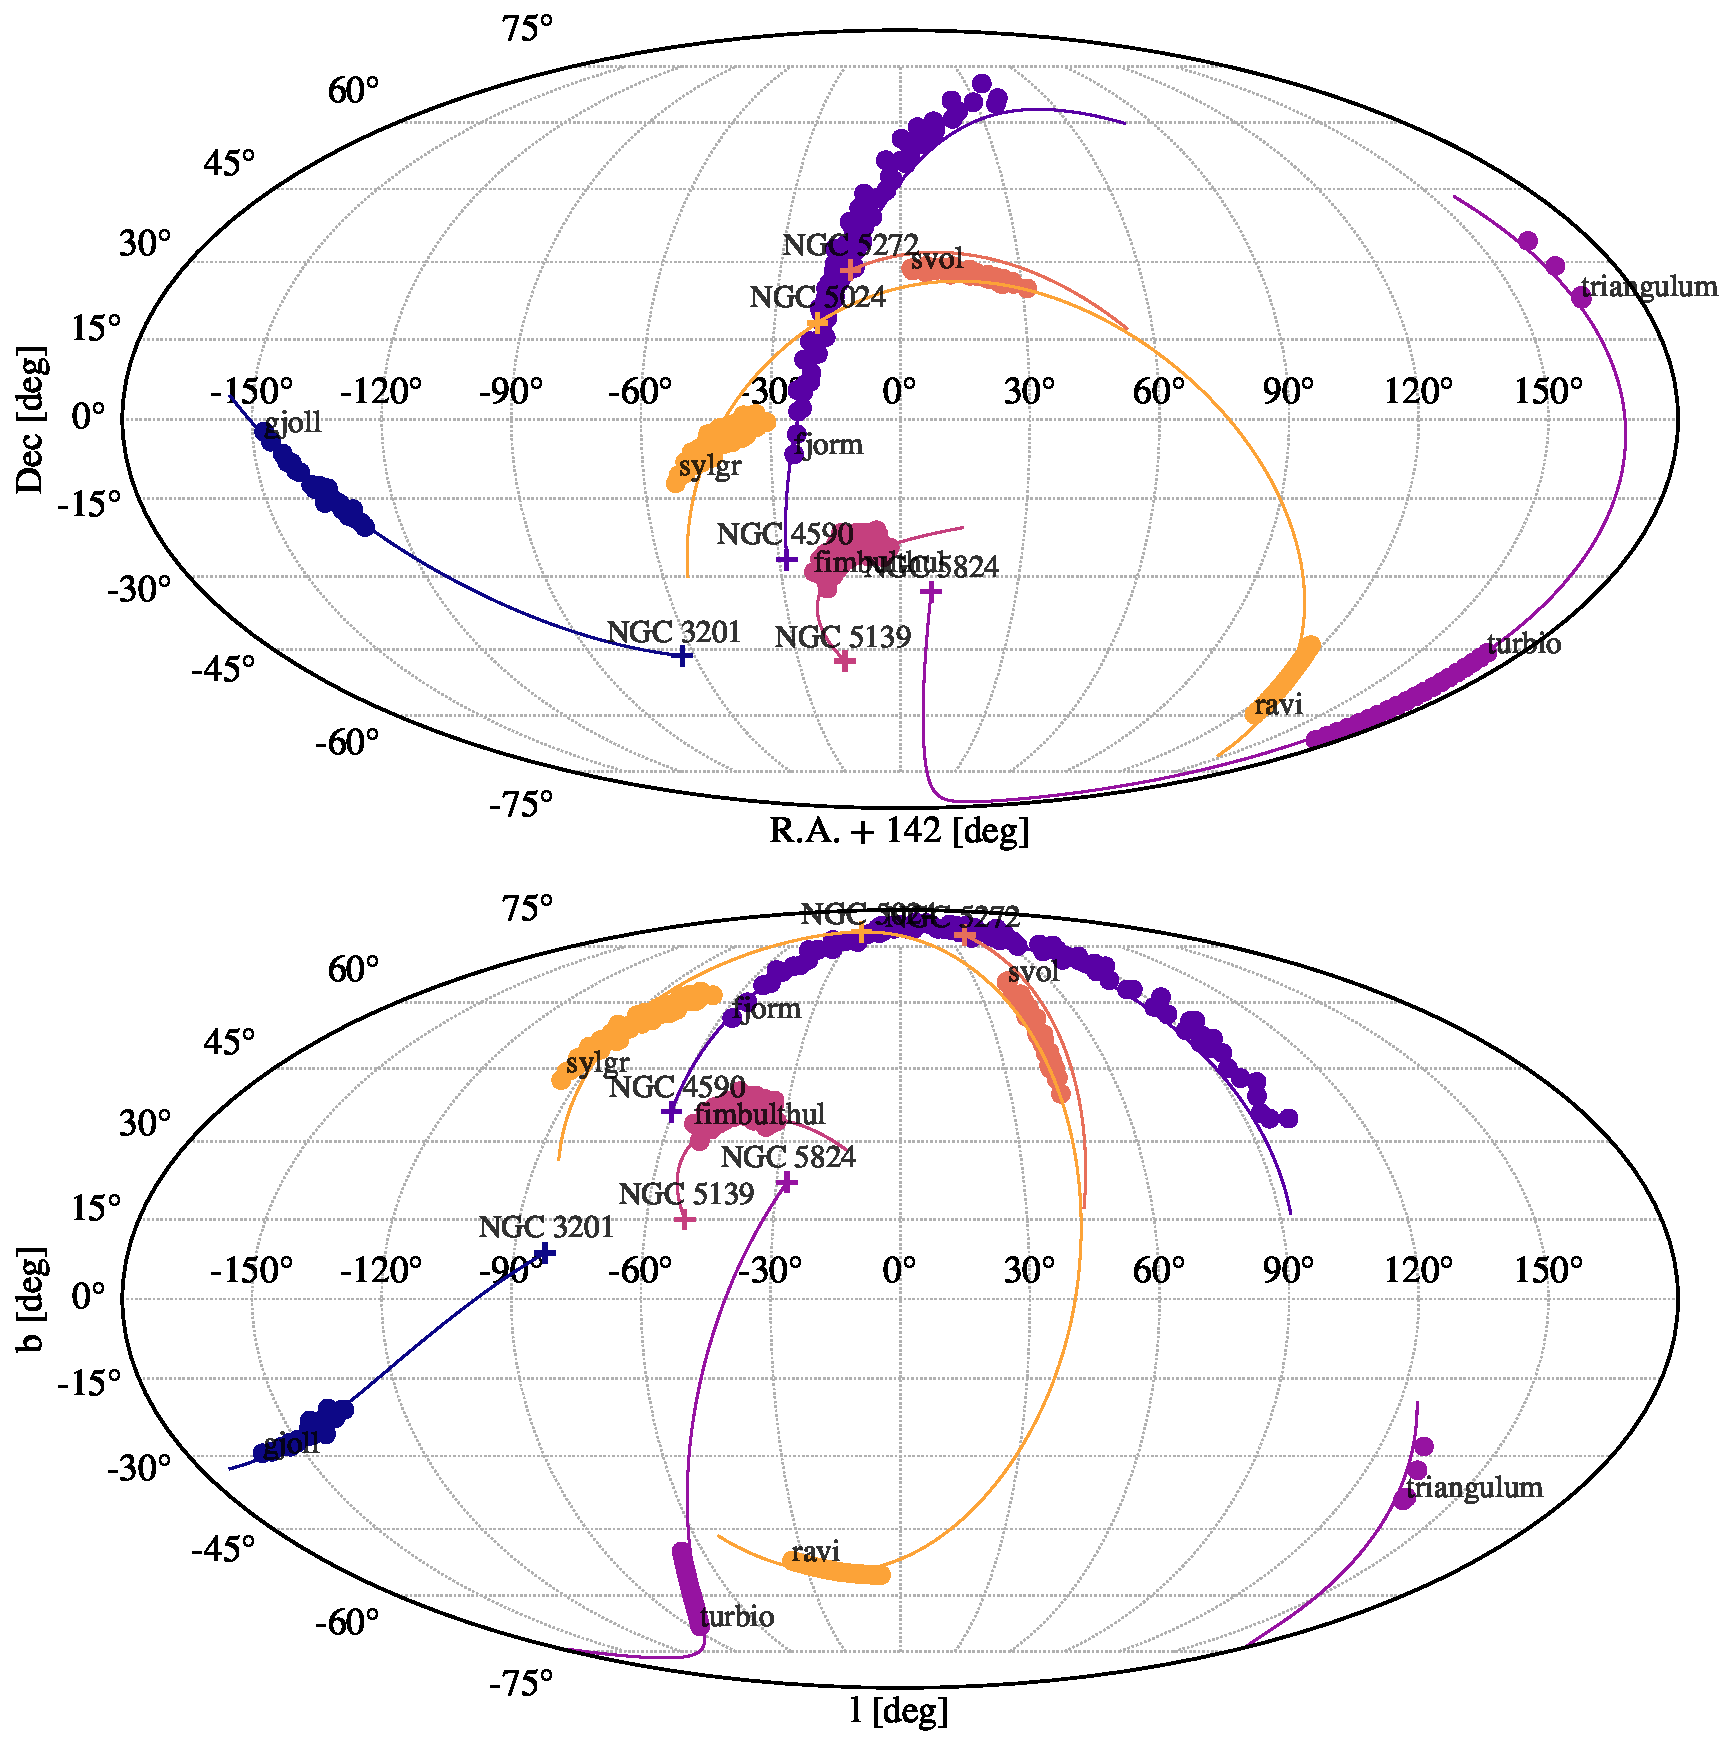
\includegraphics[width=0.9\textwidth]{sky_orbits.pdf}
\end{center}
\caption{
Sky positions of stellar streams (circles) and globular clusters (crosses) that have similar orbital energies and angular momenta (see Figure~\ref{fig:elz}), shown in the equatorial coordinates in the top and galactic at the bottom.
Despite being spatially separated, these clusters are likely stream progenitors because their orbits (lines) connect them to the streams.
}
\label{fig:sky}
\end{figure*}

Finally, Triangulum and Willka Yaku form a distinct association on highly prograde, high energy orbits.
This region of phase space is occupied by stars from the Cetus stream \citep{yuan2019}.
Cetus is a $\approx2\,\deg$ wide stream spanning both hemispheres \citep[the southern portion of the stream was identified as the Palca overdensity]{newberg2009, chang2020}.
Triangulum and Willka Yaku also overlap with Cetus spatially, but they are each only $0.25\deg$ wide.
This suggests that Triangulum and Willka Yaku are dissolved globular clusters that were brought into the Milky Way by the progenitor of the Cetus stream.

These results imply that the original host galaxy for a large fraction of stellar streams in the Galactic halo was not the Milky Way, but one of its lower-mass progenitors.
Tentative associations of streams and their host galaxies are listed in Table~\ref{table}.



\begin{deluxetable}{l c c c c}
\tablehead{
Name & Host Galaxy & Progenitor & Type & \feh
}
\decimals
\startdata
Aliqa Uma & Sagittarius & nan & GC & -2.4\\ 
ATLAS & Sagittarius & nan & GC & -2.4\\ 
Elqui & itself & itself & DG & -2.2\\ 
Fimbulthul & Gaia Enceladus & NGC 5139 & GC & -1.5\\ 
Fj\"{o}rm & Sagittarius & NGC 4590 & GC & -2.2\\ 
GD-1 & Sequoia / Arjuna / I'itoi & nan & GC & -2.3\\ 
Gj\"{o}ll & Sequoia & NGC 3201 & GC & -1.5\\ 
Indus & (Gaia Enceladus) & itself & DG & -2.1\\ 
Jhelum & (Gaia Enceladus) & itself & DG & -2.1\\ 
Leiptr & Sequoia & nan & GC & -1.6\\ 
Ophiuchus & Gaia Enceladus & nan & GC & -1.9\\ 
Phlegethon & Sequoia & nan & GC & -1.6\\ 
Phoenix & Helmi/Wukong & nan & GC & -2.7\\ 
Ravi & Helmi/Wukong & NGC 5024 & GC & -1.6\\ 
Slidr & Sagittarius & nan & GC & -1.7\\ 
Sv\"{o}l & in situ & NGC 5272 & GC & -1.1\\ 
Sylgr & Helmi/Wukong & NGC 5024 & GC & -2.7\\ 
Triangulum & Cetus & NGC 5824 & GC & -1.9\\ 
Turbio & Cetus & NGC 5824 & GC & nan\\ 
Turranburra & Sagittarius & nan & GC & nan\\ 
Wambelong & Sequoia / Arjuna / I'itoi & nan & GC & -2.2\\ 
Willka Yaku & Cetus & nan & GC & nan\\ 
Ylgr & Sequoia / Arjuna / I'itoi & nan & GC & -1.9\\ 

\enddata
\caption{
The original progenitors and host galaxies of stellar streams in the Milky Way.
Tentative host galaxies are placed in parentheses.
}
\label{table}
\end{deluxetable}


\subsection{Association with globular clusters}
\label{sec:progenitors}
In this section we explore whether globular cluster progenitors of stellar streams can be identified based on their proximity in the phase space.
Inspection of the right panel of Figure~\ref{fig:elz} reveals several cases in which a globular cluster is very close in $E-L_Z-L_\perp$ space to one or more stellar streams.
Figure~\ref{fig:sky} shows the sky positions of six strongest associations, with the equatorial coordinates in the top panel and Galactic in the bottom panel.
In this figure the globular clusters are shown as crosses and stream stars as circles (associated objects have the same color).
Starting with the 6D positions from \citet{baumgardt2019} we integrated orbits of these clusters and in all cases found that they clearly connect to stellar streams (shown as lines of matching colors in Figure~\ref{fig:sky}).
The connections between Fimbulthul and NGC~5139 (Omega Cen), and Gj\" oll and NGC~3201 have been previously identified \citep[respectively]{ibata2019b, hansen2020}.
These results suggest that associations between a globular cluster and a stellar stream, where the stream does not connect directly to the cluster, are common in the Milky Way (eight out of 23 streams).

These associations challenge the established picture in which tidal tails are developed symmetrically around globular clusters through steady mass loss \citep[e.g.,][]{kuepper2010}.
In several cases, the stream and the cluster are on opposite sides of the Galactic disk (bottom panel).
The high contamination rate and extinction at low Galactic latitudes may be preventing a complete mapping of Gj\" oll, Turbio and Ravi.
Furthermore, parts of stellar streams might be missing due to observational limitations, such as footprints of photometric surveys in the case of Ravi, Triangulum, and Turbio, and the varying degree to which streams stand out against the bulk of the Milky Way stars in proper motions (for Fimbulthul, Fj\" orm, Gj\" oll, Sv\" ol, and Sylgr).
Dedicated searches along the orbital paths shown in Figure~\ref{fig:sky} with more precise Gaia EDR3 proper motions \citep{edr3} and extended photometric catalogs \citep{decals} should determine whether the stream gaps along these clusters' orbits are physical or a selection effect.

Episodic mass loss from a globular cluster is a physical mechanism that can explain the uneven density along these clusters' orbits.
These episodes can be induced in pericentric passages \citep{general_stripping_ref}, disk crossing \citep{dehnen2004}, encounters with other structures \citep{?}, core collapse \citep{?}, or upon accretion onto the Milky Way \citep{?}.
In all of these scenarios we still expect tails to form symmetrically around the cluster, but we identify both the leading and the trailing debris only with NGC~5024 (Sylgr and Ravi).
A search for the leading/trailing counterparts of other detected streams is needed.

While the degree to which globular clusters' orbits match stellar streams in Figure~\ref{fig:sky} is striking, the orbits in many cases do not exactly trace the locations of the streams.
Notably, the entire tracks of Sv\" ol and Triangulum are offset from the orbits of their matching clusters, while both Sylgr and Ravi are misaligned with the orbit of NGC~5024.
Such discrepancies can arise if the cluster's orbit has evolved since forming streams.  {\color{red} this should be phrased more precisely.  I think you mean that the orbit is possibly not well-described by a point-mass in a static potential?} 
Matching in detail the streams and clusters we associated should provide strong constraints on the global structure and evolution of the Milky Way's gravitational potential.

% weekend:
% - sample orbital uncertainties of gcs and show

\section{Discussion}
\label{sec:discussion}
- summary
% implications for galaxy formation:
- meshes well w the accretion picture from stars, gc
% - speculate on the lower energy than stars, gcs -- those got disrupted first?
- put table

bc the progenitor identified:
- streams long -- more informative \citep{bh2018}
- had a chance to record the Galaxy evolving
- asymmetry - mond, scattering by chaos

special bc accreted:
- should have similar elz, clustering == metric of the grav potential
- difference in velocity dispersion depends whether cusp / core for dwarf streams, aggregate different in gc streams

future outlook

\vspace{0.5cm}
It is a pleasure to thank 

\software{
\package{Astropy} \citep{astropy, astropy:2018},
\package{gala} \citep{gala},
\package{IPython} \citep{ipython},
\package{matplotlib} \citep{mpl},
\package{numpy} \citep{numpy},
\package{scipy} \citep{scipy}
}

\bibliographystyle{aasjournal}
\bibliography{elz}


\end{document}